\documentclass{report}
\usepackage[spanish]{babel}
\usepackage[utf8]{inputenc}
\usepackage{graphicx, tabularx}

\begin{document}

    \begin{titlepage}
        \centering
        
\includegraphics[width=0.6\textwidth]{./img/miscelanio/logo.jpg}\\
        \vspace{1cm}
        \LARGE Análisis y Diseño de Sistemas de Información\\
        \vspace{0.5cm}
        \Large Ingeniería Informática de Gestión y Sistemas de Información\\
        \vspace{3cm}
        \Huge Biblioteca\\
        \vspace{2.5cm}
        \Large Autores:\\
        \vspace{0.2cm}
        \large Xabier Gabiña\\
        \large Janire Veganzones\\
        \large Ainhize\\
        \large Javier Criado\\
        \large Kepa Reches\\
        \large Jon Valdes\\
        \large Mohammed El Basri Dehbi\\
        \vfill
        \today
    \end{titlepage}

    \tableofcontents
    \chapter{Changelog}
        \section{Versión 1 (2023-10-08)}
            \begin{itemize}
                \item Añadido caso de uso general
                \item Añadidos los casos de uso extendidos
            \end{itemize}   
    \chapter{Introducción}
    \chapter{Casos de Uso}
        \section{General}
        \clearpage
        \section{Extendidos}
        \clearpage
        \subsection{Gestión de reservas}
        \clearpage
        \subsection{Reseñas}
        \clearpage
        \subsection{Red de amigos}
        \clearpage
        \subsection{Administrador}
        \clearpage
        \subsection{Foros}
        \clearpage
        \subsection{Recomendaciones del sistema}
            \begin{center}
                \begin{tabular}{|p{\linewidth}|}
                    \hline
                    \textbf{Responsable:} Xabier Gabiña\\
                    \hline
                    \begin{minipage}{\textwidth}
                        \centering
                        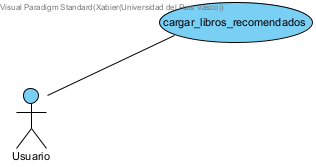
\includegraphics[width=0.4\textwidth]{./img/casos_uso/recom_lib.png}
                    \end{minipage}\\
                    \hline
                    \textbf{Nombre:} Ver libros recomendados\\
                    \hline
                    \textbf{Descripción:} Muestra una lista en la parte superior del catálogo mostrando los libros con más préstamos del sistema en funcion de los gustos del usuario.\\
                    \hline
                    \textbf{Actores:} Usuario\\
                    \hline
                    \textbf{Precondiciones:} Estar identificado en el sistema\\
                    \hline
                    \textbf{Requisitos no funcionales:} El Usuario debe de haber tenido al menos una pelicula alquilada\\
                    \hline
                    \textbf{Flujo de Eventos:}
                    \begin{enumerate}
                        \item El Usuario entra en el catalogo para ver las peliculas disponibles.
                        \item Se le muestra en la parte superior de la pantalla una serie de peliculas basadas en los generos y peliculas que consume el usuario.
                    \end{enumerate}\\
                    \hline
                    \textbf{Poscondiciones:} Ninguna\\
                    \hline
                    \textbf{Interfaz Gráfica:}\\
                    \begin{minipage}{\textwidth}
                        \centering
                        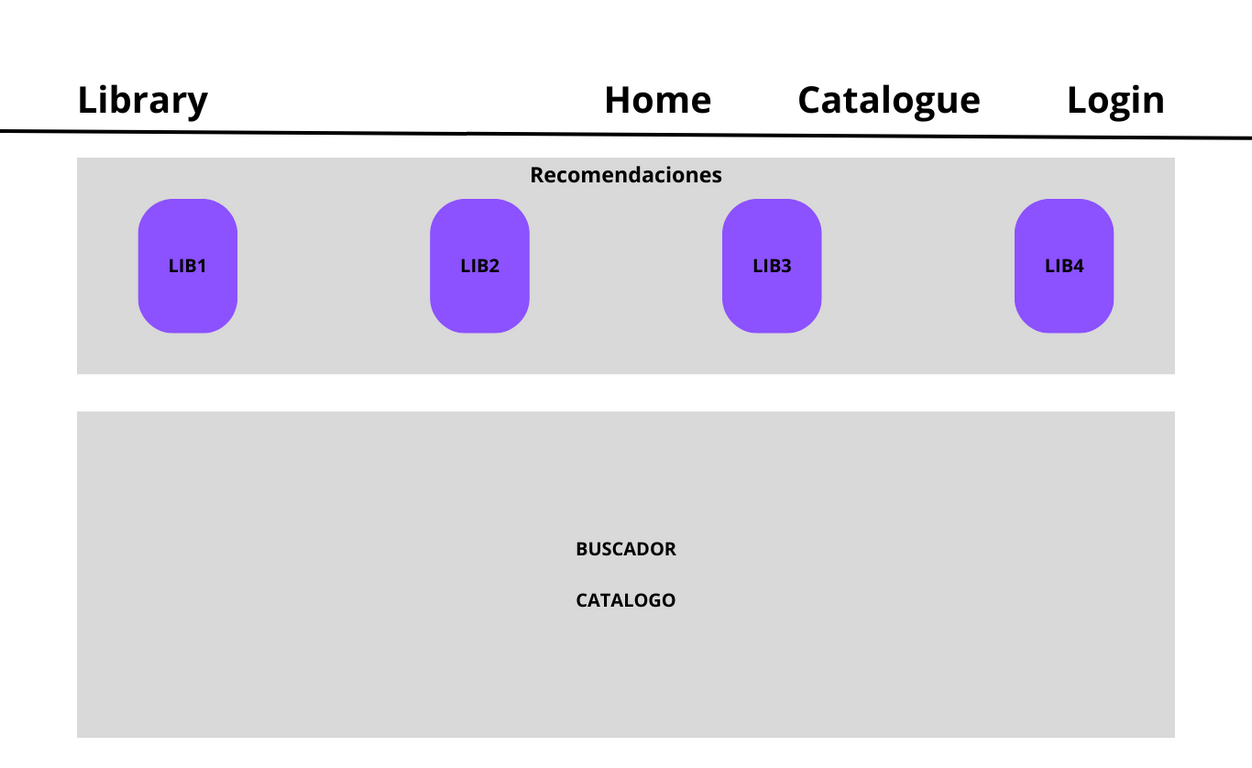
\includegraphics[width=0.9\textwidth]{./img/grafico/recom_lib.png}
                    \end{minipage}\\
                    \hline
                \end{tabular}
            \end{center}
        \clearpage
        \subsection{Recomendaciones de amigos}
    \chapter{Conclusiones} 

\end{document}